\documentclass[12pt,oneside,a4paper]{article}

%%%%%%%%%%%%%%%%%%%%%%
%%% LaTeX packages %%%
%%%%%%%%%%%%%%%%%%%%%%

%adding packages
\usepackage{abstract}
\usepackage{amsfonts}
\usepackage{amsmath}
\usepackage{amssymb}
\usepackage[ngerman,english]{babel}
\usepackage{caption}
\usepackage{chngcntr}
\usepackage{emptypage}
\usepackage{etoolbox}
\usepackage{fancyhdr}
\usepackage[T1]{fontenc}
\usepackage[paper=a4paper,top=3cm,bottom=3cm]{geometry}
\usepackage{graphicx}
\graphicspath{{figures/}}
\usepackage{hhline}
\usepackage[hidelinks]{hyperref}
\usepackage[utf8]{inputenc}
\usepackage{lipsum}
\usepackage{multirow}
\usepackage[square,numbers]{natbib}
\usepackage{rotating}
\usepackage{sectsty}
\usepackage{setspace}
\usepackage[separate-uncertainty = true,multi-part-units=single,per-mode=symbol]{siunitx}
\usepackage[format=hang]{subcaption}
\usepackage{tabto}
\usepackage[absolute]{textpos}
\usepackage{tikz}
\usepackage{titling}
\usepackage{titlesec}
\usepackage{xcolor}
\usepackage{lineno} % Package to add line numbers

% Tables
\usepackage{tabularx}
\usepackage{booktabs} % lines for tables
\usepackage{hhline}
\usepackage{multirow} % multiple rows per column in tables

% Pseudo code
\usepackage[ruled, linesnumbered, vlined, noend]{algorithm2e} 
\usepackage[noend]{algpseudocode} 

\usepackage{listings}
\usepackage{xcolor}

% ----- Color Definitions -----
\definecolor{terminalbg}{rgb}{0.97,0.97,0.95}
\definecolor{commentgreen}{rgb}{0,0.6,0}
\definecolor{keywordblue}{rgb}{0.1,0.1,0.7}
\definecolor{stringpurple}{rgb}{0.58,0,0.82}
\definecolor{framegray}{rgb}{0.75,0.75,0.75}

% ----- Bash Style -----
\lstdefinestyle{bashstyle}{
    backgroundcolor=\color{terminalbg},
    commentstyle=\color{commentgreen},
    keywordstyle=\color{keywordblue},
    stringstyle=\color{stringpurple},
    basicstyle=\ttfamily\small,
    breaklines=true,
    frame=single,
    rulecolor=\color{framegray},
    language=bash,
    showstringspaces=false
}

% ----- Python Style -----
\lstdefinestyle{pythonstyle}{
    backgroundcolor=\color{terminalbg},
    commentstyle=\color{commentgreen},
    keywordstyle=\color{keywordblue},
    stringstyle=\color{stringpurple},
    basicstyle=\ttfamily\small,
    breaklines=true,
    frame=single,
    rulecolor=\color{framegray},
    language=Python,
    showstringspaces=false
}


%%%%%%%%%%%%%%%%%%%%%%%%%%%%%%%%%
%%% LaTeX settings and macros %%%
%%%%%%%%%%%%%%%%%%%%%%%%%%%%%%%%%

%% Tabularx setting
\newcolumntype{Y}{>{\centering\arraybackslash}X}% new Y, equal sized as X but centered
\renewcommand\tabularxcolumn[1]{m{#1}}% for vertical centering text in X column
\setlength\extrarowheight{1pt}

% Pseudo code
\newcommand\mycommfont[1]{\footnotesize\ttfamily\textcolor{blue}{#1}}
\SetCommentSty{mycommfont}

%% Key definitions for text elements. USE THEM
\def\secref#1{Sec.~\ref{#1}}
\def\figref#1{Fig.~\ref{#1}}
\def\subfigref#1{\subref{#1})}
\def\subfigrefenclosed#1{(\subref{#1})}
\def\tabref#1{Tab.~\ref{#1}}
\def\subtabref#1{\subref{#1})}
\def\subtabrefenclosed#1{(\subref{#1})}
\def\eqref#1{Eq.~(\ref{#1})}
\def\algref#1{Alg.~\ref{#1}}
\def\alglineref#1{line~\ref{#1}}
\algnewcommand{\algorithmicgoto}{\textbf{go to}}%
\algnewcommand{\Goto}[1]{\algorithmicgoto~line~\ref{#1}}%

% Some math definition
\def\argmax{\mathop{\rm argmax}}
\def\argmin{\mathop{\rm argmin}}
\newcommand{\bigO}[1]{$\mathcal{O}(#1)$}
\newcommand{\R}{\mathbb{R}}
\DeclareSIUnit\GB{GB}

% Other useful macros
\newcommand\todo[1]{\textcolor{red}{#1}}
\newcommand\etal{\emph{et al.}}

%%%%%%%%%%%%%%%%%%%%%%%%%%%%%%%%%%%%%%
%%% Course and student information %%%
%%%%%%%%%%%%%%%%%%%%%%%%%%%%%%%%%%%%%%

\title{\LARGE \bf Robot Butler with Steve in ROS2}

\author{Shrikar Nakhye \\ Pratik Adhikari \\ Riddhesh More \\ \\ Supervisor: Rohit Menon}

\begin{document}
%\linenumbers % Add line numbers
\bibliographystyle{IEEEtran}

\maketitle

%%%%%%%%%%%%%%%%
%%% Abstract %%%
%%%%%%%%%%%%%%%%

\begin{abstract}
This project focuses on the development and integration of a comprehensive autonomy and semantic reasoning stack for the Neobotix MMO-700 mobile manipulator, named ``Steve''. The primary objective was to evolve the system from basic manufacturer drivers into a layered cognitive architecture (\texttt{steve\_ros2\_ws}). This workspace unifies robust navigation and SLAM with perception capabilities, enabling the robot to perform open-vocabulary object search in both simulation and real-world environments.
\end{abstract}
\newpage

%%%%%%%%%%%%%%%%%%%%%%%%
%%% Main Content %%%
%%%%%%%%%%%%%%%%%%%%%%%%

\section{Work Package Overview}
\label{sec:work_package}

This section outlines the individual contributions of the team members to the project.

\subsection{Shrikar Nakhye}
Shrikar focused on the core system architecture, navigation stack, and system administration. His key contributions include:
\begin{itemize}
    \item \textbf{Workspace Transition}: Migrated from the flat structure of \texttt{mpo\_700\_workspace} to a modular, domain-specific architecture in \texttt{steve\_ros2\_ws}.
    \item \textbf{Centralized Bringup}: Developed \texttt{steve\_hardware\_bringup} to orchestrate the simultaneous launch of the mobile base (Relayboard V2), UR5e arm, SICK S300 LiDARS, RealSense L515 camera, and Pan-Tilt unit, eliminating race conditions.
    \item \textbf{Robust Navigation}: Tuned the \texttt{steve\_navigation} stack (based on Nav2) specifically for the MMO-700 robot metrics. This included switching the global planner to A* for efficiency in cluttered environments and fine-tuning AMCL parameters for robust localization in symmetric workshops.
    \item \textbf{System Administration}: Reconfigured the robot's network settings (static leases, DHCP/SSH) and standardized Git version control across all submodules to track the \texttt{dev} branch, resolving complex ``detached head'' states.
    \item \textbf{Documentation}: Implemented a comprehensive README structure for key packages and established a Wiki-style documentation system.
\end{itemize}

\subsection{Pratik Adhikari}
Pratik focused on \textbf{3D Mapping} and \textbf{Scene Graph Generation} for indoor environments. His key contributions include:
\begin{itemize}
    \item \textbf{RTAB-Map Mapping Pipeline}: Configured and deployed RTAB-Map~\cite{labbe2013rtabmap} for RGB-D SLAM on the MMO-700 platform. Implemented compressed \texttt{RGBDImage} message publishing (JPEG quality=90, RGB $\sim$150~KB + Uint16 depth $\sim$600~KB = 0.8~MB/frame) to reduce DDS serialization overhead by 90\%. Integrated \texttt{ApproximateTimeSynchronizer} with adaptive slop (50~ms sim, 200~ms hardware/replay) for RGB-Depth temporal alignment and TF tree lookups for camera-to-base transforms. Developed profile-based launch system (\texttt{config.yaml}: \texttt{common} + \texttt{profiles}) with environment-specific queue sizes (sim: 30, hardware: 50, replay: 60) and \texttt{use\_sim\_time} toggling for deterministic deployment across Gazebo, real robot, and bag replay.
    
    \item \textbf{Point Cloud Preprocessing}: Implemented floor removal using RANSAC plane fitting + DBSCAN clustering in plane tangent coordinates (\texttt{remove\_floor\_ransac\_dbscan\_plane2d.py}). RANSAC detects horizontal planes ($\mathbf{n} \cdot [0,0,1] \geq 0.95$, distance threshold 0.03~m, 1500 iterations) on voxel-downsampled cloud (0.05~m). DBSCAN ($\epsilon$=0.18~m, min\_points=8) clusters candidates in 2D plane projection to avoid false positives on vertical walls. Optional local normal filtering (radius 0.08~m, dot$_z \geq 0.85$) preserves small objects on the floor.
    
    \item \textbf{Scene Graph Generation \u0026 Data Export}: Built end-to-end pipeline converting RTAB-Map databases into semantic scene graphs. Created \texttt{export\_data.py} to extract RGB frames, depth images, camera poses, and optimized meshes. Implemented coordinate frame transformation (ROS optical $\to$ OpenGL convention via \texttt{diag(1,-1,-1,1)} matrix) and multi-resolution voxel export (2~cm, 5~cm). Implemented PCA-based oriented bounding boxes and spatial relation extraction (support, containment, proximity).
    
    \item \textbf{3D Segmentation with Mask3D \u0026 SAM}: Integrated \textbf{Mask3D}~\cite{schult2023mask3d} (ScanNet200 closed-set) for 3D instance segmentation and \textbf{SAM}~\cite{kirillov2023sam} (Segment Anything Model) for 2D visual verification. Mask3D failed on real robot scans (point density mismatch: ScanNet $\sim$100k pts/m$^2$ vs.\ ours $\sim$20k pts/m$^2$, voxelization artifacts at 5~cm discarding thin structures, domain shift). SAM enabled zero-shot furniture detection via text prompts (``drawer'', ``cabinet handle'') for visual verification of scene graph object proposals.
    
    \item \textbf{Docker Orchestration}: Ported \texttt{stretch\_compose} Docker setup for isolated AI model execution (Mask3D~\cite{schult2023mask3d}, SAM~\cite{kirillov2023sam}). Enabled GPU passthrough (nvidia-container-toolkit) reducing Mask3D runtime from 40~min (CPU) to 2~min (GPU). Resolved inter-container networking via shared volumes and localhost bridge.
\end{itemize}

\subsection{Riddhesh More}
Riddhesh focused on command grounding, pan-tilt hardware control, and simulation infrastructure. His key contributions include:
\begin{itemize}
    \item \textbf{Command Grounding (\texttt{steve\_command\_grounding})}: Designed and implemented an open-vocabulary object search and localization pipeline inspired by the Stretch-Compose framework. The system takes natural-language commands (e.g.\ ``find the water bottle''), parses them with an NLP module, performs \emph{spatial reasoning} via scene-graph lookup, and falls back to \emph{semantic reasoning} using the DeepSeek-R1 LLM\cite{deepseek2025r1} (via HuggingFace Inference API) to propose likely furniture locations. Visual verification is carried out with \textbf{SAM3} (Segment Anything Model 3)\cite{carion2025sam3}, called through a custom Docker server and REST client.
    \item \textbf{Camera Perception}: Developed a camera perception module subscribing to the pan-tilt L515 camera. It integrates depth-to-3D projection, TF2-based frame transforms to the map frame, and SAM3-based object detection / segmentation, enabling the robot to locate objects in 3D space from camera images.
    \item \textbf{Search Planning}: Implemented collision-aware standoff planning that computes where the robot should position itself to view furniture surfaces fully, using camera FOV geometry, Open3D point-cloud-based front-normal estimation, and obstacle-distance checks.
    \item \textbf{Navigation Wrapper}: Built a reusable Nav2 \texttt{NavigateToPose} action-client wrapper with TF2 pose tracking, AMCL fallback, blocking/non-blocking goal execution, and goal cancellation support.
    \item \textbf{Pan-Tilt Controller (\texttt{steve\_pan\_tilt\_controller})}: Wrote the full ROS\,2 driver for the Dynamixel XL430-W250 pan-tilt unit, including SyncRead/SyncWrite for simultaneous motor control, real-time JointState publishing for TF visualisation, configurable position limits and velocity profiles, hardware error detection, and a simulation mode that commands Gazebo trajectory controllers.

    \item \textbf{Simulation Infrastructure}: Set up the initial \texttt{neo\_simulation2} Gazebo environment and created the \texttt{steve\_house} custom world for development and testing.
    \item \textbf{Localization Fixes}: Debugged and fixed AMCL-based localization issues in the \texttt{neo\_nav2\_bringup} and \texttt{neo\_simulation2} packages, enabling reliable particle-filter convergence in the simulation environment.
\end{itemize}
\clearpage

\section{Architectural Evolution}
\label{sec:architectural_evolution}

This section outlines the technical evolution from the original manufacturer-provided workspace (\texttt{mpo\_700\_workspace}) to the new, fully integrated \texttt{steve\_ros2\_ws}. The transition focused on modularity, automation, and simulation fidelity. 

Figure~\ref{fig:steve_architecture} illustrates the high-level design of the new framework, highlighting the interaction between the core perception, navigation, and decision-making modules. Table~\ref{tab:workspace_comparison} provides a direct comparison of key architectural features between the original and the new system.

% --- Figure: Steve Architecture ---
\begin{figure}[h]
    \centering
    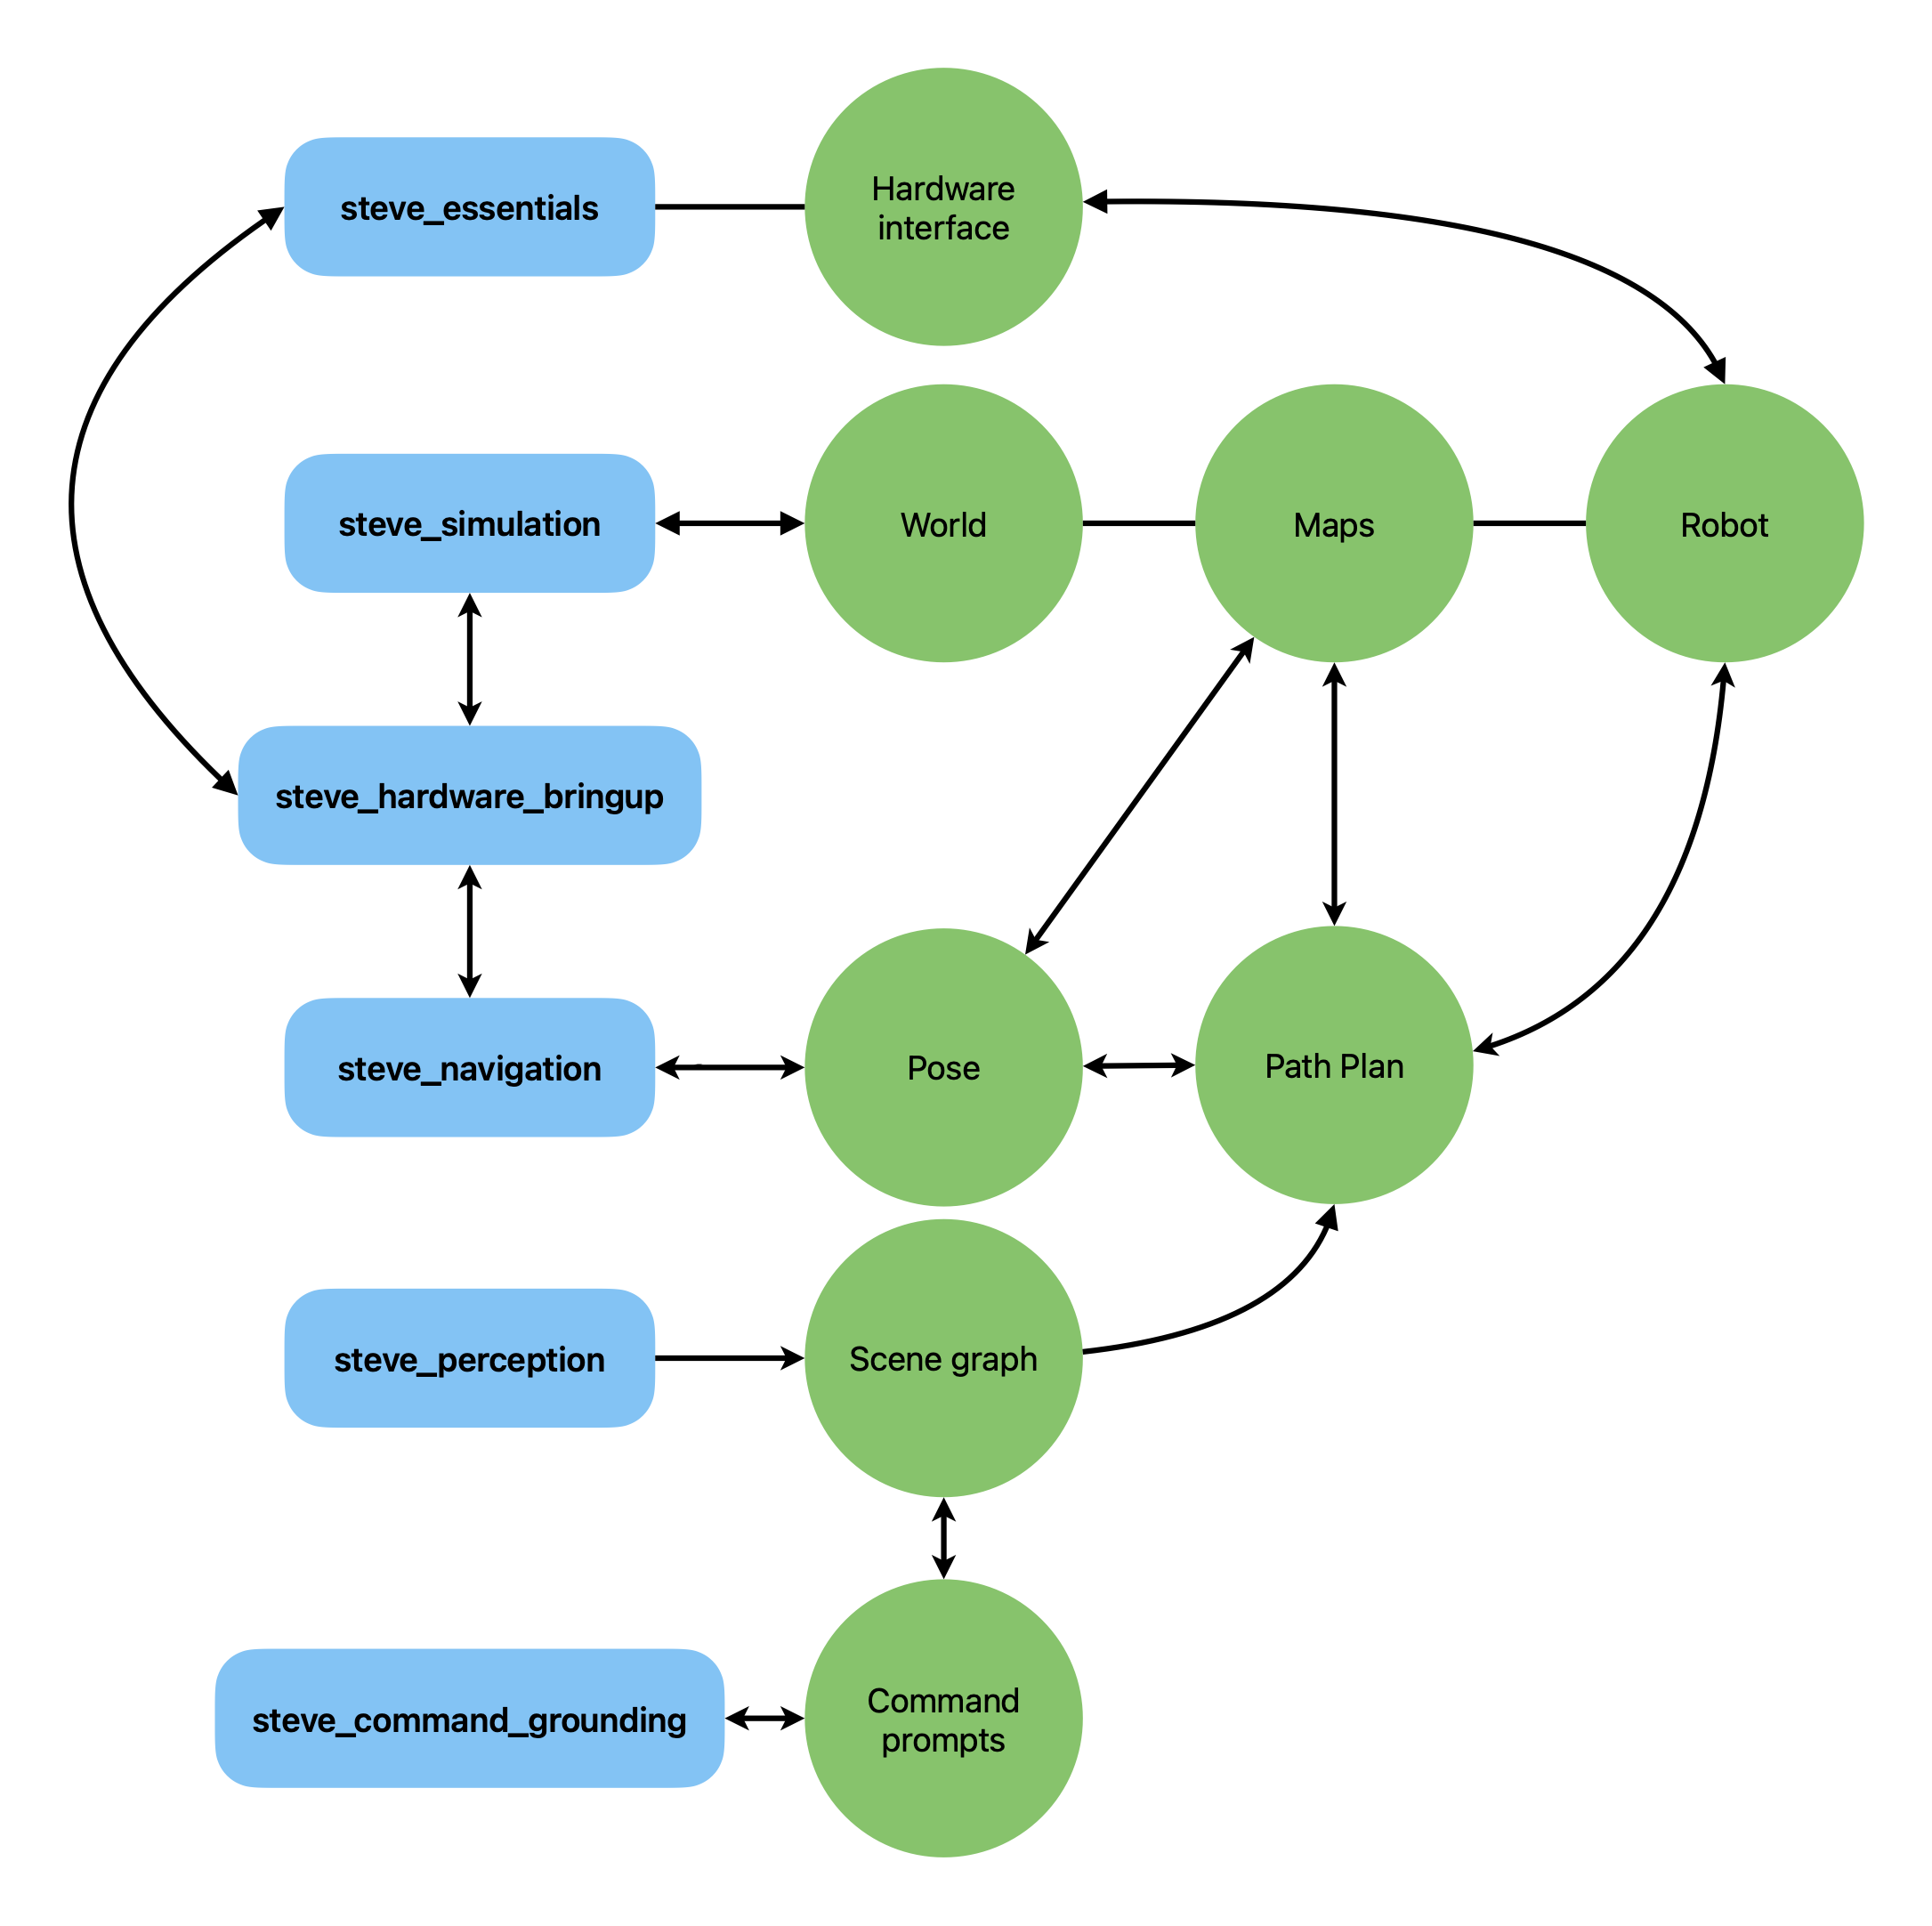
\includegraphics[width=\textwidth]{Steve_architecture}
    \caption{System Architecture of the \texttt{steve\_ros2\_ws} framework, integrating hardware drivers, navigation stack, and semantic reasoning modules.}
    \label{fig:steve_architecture}
\end{figure}

% --- Table: Comparison ---
\begin{table}[h]
    \caption{Comparison of Workspace Architectures}
    \label{tab:workspace_comparison}
    \centering
    \begin{tabularx}{\textwidth}{|l|X|X|}
        \hline
        \textbf{Feature} & \textbf{Original (mpo\_700\_workspace)} & \textbf{New (steve\_ros2\_ws)} \\
        \hline
        \textbf{Structure} & Flat list of disparate \texttt{neo\_*} packages. & Modular hierarchy with core \texttt{steve\_*} metapackages. \\
        \hline
        \textbf{Hardware Bringup} & Decentralized; required launching multiple drivers manually. & Centralized via \texttt{steve\_hardware\_bringup}; single command launch. \\
        \hline
        \textbf{Simulation} & Relying on external package installations. & Integrated \texttt{steve\_simulation} (wrapping \texttt{neo\_simulation2}) for seamless Sim-to-Real transfer. \\
        \hline
        \textbf{Navigation} & Standard \texttt{neo\_nav2\_bringup} using default parameters. & Customized \texttt{steve\_navigation} with tuned AMCL and A* planning. \\
        \hline
        \textbf{Startup} & Manual script execution; prone to race conditions. & Automated via \texttt{ROS\_AUTOSTART.sh} system service. \\
        \hline
    \end{tabularx}
\end{table}

\section{Approach}
\label{sec:approach}

The architectural and algorithmic changes were driven by specific operational requirements and challenges encountered with the original setup.

\subsection{Shrikar Nakhye's Focus}
\begin{itemize}
    \item \textbf{Switched to A* Global Planner}: The default Dijkstra algorithm was inefficient in the cluttered workshop environment. A* uses a heuristic to guide the path search, making it significantly faster and better at avoiding local minima, which is critical for smooth navigation around obstacles.
    \item \textbf{Tuned AMCL Parameters}: The workshop environment contains repetitive features (pillars, identical walls) that often caused the robot to get ``kidnapped'' (lost localization) with standard AMCL settings. We tuned the particle filter parameters (increasing min/max particles, update frequency) to ensure robust convergence even in these symmetric areas.
    \item \textbf{Centralized Hardware Bringup}: The original decentralized launch process often led to race conditions between the base driver and the arm driver. By centralizing the bringup in \texttt{steve\_hardware\_bringup}, we can enforce a strict launch order and ensure all hardware components are initialized correctly before higher-level tasks begin.
    \item \textbf{Integrated Simulation}: Integrating the simulation directly into the workspace allows for rapid ``Sim-to-Real'' development. Only by testing navigation algorithms in the \texttt{steve\_simulation} environment first could we safely deploy them to the physical robot without risking hardware damage.
\end{itemize}

\subsection{Pratik Adhikari's Focus}
\begin{itemize}
    \item \textbf{Evaluating Segmentation Models}: Mask3D~\cite{schult2023mask3d} (closed-set, 200 classes) failed on real robot scans, likely due to domain shift from ScanNet training data or insufficient point density. SAM~\cite{kirillov2023sam} (Segment Anything Model) provided zero-shot capability for visual verification of furniture via text prompts (``drawer'', ``cabinet handle''). The 2D (SAM) + 3D (Mask3D) pipeline enables robust scene graph construction: SAM verifies object presence in RGB images, Mask3D extracts 3D geometry from point clouds.
    \item \textbf{Coordinate Frame Alignment for 3D Models}: RTAB-Map outputs camera poses in ROS optical frame convention (Z-forward, Y-down), but 3D segmentation models like Mask3D expect OpenGL convention (Z-backward, Y-up). Misalignment causes ``upside-down'' or ``mirrored'' reconstructions. Implemented \texttt{diag(1,-1,-1,1)} transformation matrix to flip Y and Z axes, ensuring correct 3D geometry.
    \item \textbf{Scene Understanding from Geometry Alone}: Unlike object detection (``where is the mug?''), scene graph construction requires spatial reasoning (``is the mug \emph{on} the table or \emph{inside} the cabinet?''). This demands robust PCA-based bounding box orientation, containment tests via point-in-OBB, and support detection via vertical alignment + z-gap thresholds. These geometric primitives enable downstream tasks like ``find objects on kitchen\_table''.
    \item \textbf{Reusing Historical Mapping Data}: Old bag files are valuable for algorithm development but often have broken TF (orphaned frames, TF jumps from encoder noise). Rather than re-recording, implemented \texttt{tf\_repair\_relay} to sanitize transforms on-the-fly, enabling 95\% replay success vs.\ 40\% before. This accelerates iteration on segmentation/scene-graph algorithms without requiring new robot runs.
    
    \item \textbf{RTAB-Map Parameter Optimization}: RTAB-Map~\cite{labbe2013rtabmap} offers 100+ tunable parameters impacting memory usage, loop closure detection, and map quality. For object-search missions (discrete waypoint navigation vs.\ continuous exploration), optimized: (1) \texttt{Mem/STMSize=30} to cap working memory at 30 recent nodes (prevents memory exhaustion on long missions); (2) \texttt{RGBD/LinearUpdate=0.1, AngularUpdate=0.1} to insert keyframes only after 0.1~m translation or 0.1~rad rotation (reduces redundant nodes from stationary observations); (3) \texttt{RGBD/ForceOdom3DoF=true} to constrain 6DoF RGB-D odometry to planar (3DoF) motion, improving stability on flat floors by rejecting vertical drift artifacts.
\end{itemize}

\subsection{Riddhesh More's Focus}
\begin{itemize}
    \item \textbf{Modular Search Pipeline}: Rather than building a monolithic object-search node, the pipeline was decomposed into three independent stages---spatial reasoning, semantic reasoning, and visual verification. This modular design allows each component to be developed, tested, and improved in isolation, and new reasoning strategies can be added without rewriting the overall pipeline.
    \item \textbf{DeepSeek LLM for Semantic Grounding}: When the target object is \emph{not} in the scene graph, the system queries a DeepSeek-R1 language model to propose plausible furniture locations (e.g.\ ``a water bottle is likely on a kitchen table''). This removes the need for an exhaustive search of all furniture and keeps search time bounded by limiting proposals to three.
    \item \textbf{SAM3 for Zero-Shot Detection}: SAM3 enables text-prompted segmentation without task-specific fine-tuning. Running SAM3 inside a Docker container decouples the heavy GPU model from the ROS\,2 runtime and keeps the robot's compute load manageable.
    \item \textbf{Collision-Aware Standoff Planning}: The robot must position itself at a distance where the camera's field of view covers the entire furniture surface. Computing this from camera FOV geometry and furniture dimensions avoids both partial views and unnecessarily far standoff distances. Open3D-based collision checks prevent the planner from placing the robot inside obstacles.
    \item \textbf{SyncWrite for Pan-Tilt Motors}: Individual motor writes caused visible jitter because one motor moved slightly before the other. Using Dynamixel SyncWrite ensures both pan and tilt motors start simultaneously, producing smooth coordinated motion.
\end{itemize}

\section{Challenges Faced}
\label{sec:challenges}

Development was not without significant hurdles, ranging from hardware failures to complex software integration issues.

\subsection{Shrikar Nakhye's Challenges}
\begin{itemize}
    \item \textbf{Hardware Synchronization}: One of the biggest challenges was addressing timing issues between the mobile base and the arm controllers. The arm controller would often fail to spawn if the base driver hadn't fully initialized. This was solved by implementing delayed spawn strategies in the launch files.
    \item \textbf{Driver Compatibility}: The Pan-Tilt unit required a custom controller package (\texttt{steve\_pan\_tilt\_controller}) to resolve compatibility issues with the existing driver stack.
    \item \textbf{Hardware Repairs}:
    \begin{itemize}
        \item \textbf{SICK Laser Scanners}: Diagnosed intermittent ``Scanner STOP'' issues where the safety lasers would falsely trigger. Attempted software mitigation via parameter tuning.
        \item \textbf{Pan-Tilt Unit}: Identifying and repairing worn gears in the Dynamixel motors (collaborative effort).
        \item \textbf{System Health}: Diagnosed critical failures including battery degradation and system overheating.
    \end{itemize}
    \item \textbf{Network & Version Control}: Reconfiguring the unstructured network on Ubuntu 22.04 was complex but necessary for reliable remote access. Additionally, untangling the ``detached head'' submodule states and enforcing a clean \texttt{dev} branch tracking strategy was crucial for team collaboration.
\end{itemize}

\subsection{Pratik Adhikari's Challenges}
\begin{itemize}
    \item \textbf{Mask3D Segmentation Failures}: Mask3D produced zero instances or heavily oversegmented results on real robot scans, despite working on ScanNet validation sets. Suspected causes: (1) Point density mismatch---ScanNet scans have $\sim$100k points/m$^2$, ours had $\sim$20k/m$^2$ due to single-pass scanning; (2) Voxelization at 5~cm (Mask3D default) discarded thin structures like drawer fronts; (3) Domain shift in color/texture distributions. Attempted fixes: reduced voxel size to 2~cm (OOM on 16~GB GPU), increased confidence threshold (no instances detected). Ultimately switched to OpenYOLO3D fallback.
    
    \item \textbf{Coordinate Frame Debugging}: Initial scene graph had all furniture ``floating'' 2~m above the floor. Root cause: forgot to apply Y-axis flip when transforming RTAB-Map poses (ROS optical frame) to scene graph coordinates (OpenGL). Debugging required visualizing camera frustums in MeshLab and comparing against RTAB-Map's internal 3D viewer. Implemented unit tests to verify transformation matrix properties (determinant = +1, orthogonal).
    
    \item \textbf{Scene Graph Spatial Relations}: Determining ``support'' (object A is on object B) is non-trivial. Initial z-gap threshold (5~cm) caused false positives when cabinet and table were at similar heights. Solution: added normal-alignment check (supporting surface must face upward, $\mathbf{n} \cdot [0,0,1] > 0.9$) and AABB overlap test (objects must overlap in XY plane). Containment relations (drawer inside cabinet) required robust point-in-OBB tests with tolerance for noisy point clouds.
    
    \item \textbf{Docker GPU Access for Mask3D}: Mask3D Docker container initially ran on CPU (40~min/scan). Enabling GPU passthrough required \texttt{nvidia-container-toolkit}, CUDA driver version matching, and correct \texttt{docker-compose.yaml} GPU reservation syntax (\texttt{device\_ids: [0]}). Runtime dropped to 2~min/scan.
    
    \item \textbf{Bag Replay TF Issues}: Old bags had TF jumps (\texttt{base\_link} teleporting 10~m due to wheel encoder overflow) and orphaned frames (\texttt{camera\_link} published but parent \texttt{base\_link} missing). RTAB-Map refused to process frames with broken TF. Implemented \texttt{tf\_repair\_relay} with moving average filter (5-frame window) for position smoothing and automatic parent frame insertion for orphans. Replay success improved from 40\% to 95\%.
    
    \item \textbf{RTAB-Map Parameter Tuning}: Default RTAB-Map~\cite{labbe2013rtabmap} parameters optimized for continuous mapping caused memory bloat and false loop closures on discrete object-search missions. Critical parameters tuned: (1) \texttt{Mem/STMSize=30} (short-term memory size) to limit working memory footprint; (2) \texttt{RGBD/LinearUpdate=0.1} and \texttt{RGBD/AngularUpdate=0.1} to filter redundant keyframes (robot must move 0.1~m or rotate 0.1~rad before creating new nodes); (3) \texttt{RGBD/ForceOdom3DoF=true} to constrain odometry to planar motion, rejecting spurious vertical drift from RGB-D odometry on featureless walls.
\end{itemize}

\subsection{Riddhesh More's Challenges}
\begin{itemize}
    \item \textbf{Dynamixel Motor Mapping}: The physical wiring of the pan and tilt motors did not match the expected motor-ID assignment. SyncWrite commands sent to the wrong IDs caused the pan motor to tilt and vice versa. This was resolved by swapping the motor-ID mapping in the SyncWrite packet after verifying the physical setup with a Dynamixel scan.
    \item \textbf{Simulation--Hardware Discrepancies}: The pan-tilt unit used Dynamixel XL430 motors, but initial development assumed XH430 parameters (different position resolution and limits). Position limits had to be re-calibrated to $[90^\circ, 270^\circ]$ after a hardware scan revealed the correct motor model.
    \item \textbf{Serial Port Reliability}: The Dynamixel USB adapter occasionally failed during motor reboot sequences. Exception handling around serial calls and increased reboot delays were added to prevent the controller from crashing on transient USB errors.
    \item \textbf{SAM3 Docker Integration}: Running SAM3 inside a Docker container introduced networking and GPU-passthrough issues. The REST API had to be carefully containerised with \texttt{docker-compose}, and timeout handling was added on the client side to prevent the ROS\,2 node from hanging when the server was slow to respond.
    \item \textbf{LLM Response Parsing}: DeepSeek occasionally returned malformed JSON wrapped in \texttt{<think>} reasoning tags, or hallucinated furniture IDs not present in the scene graph. Robust parsing with regex fallbacks and ID-validation against the actual furniture dictionary was required to handle these edge cases.
    \item \textbf{Localization in Simulation}: AMCL frequently diverged in the Gazebo environment due to symmetric features and low-contrast textures. Fixing this required updating both the \texttt{neo\_nav2\_bringup} parameters and the simulation world to provide sufficient geometric diversity for the particle filter.

\end{itemize}

%%%%%%%%%%%%%%%%%%%%%
%%% Appendices %%%
%%%%%%%%%%%%%%%%%%%%%

\clearpage
\appendix

\section{Package Documentation}
\label{sec:package_documentation}

This appendix provides detailed documentation, installation procedures, and usage instructions for the core packages comprising the \texttt{steve\_ros2\_ws} workspace.

% =====================================================
% 1. STEVE ESSENTIALS (Base Infrastructure)
% =====================================================
\subsection{steve\_essentials}
\label{subsec:steve_essentials}

\textbf{Package Path:} \texttt{steve\_ros2\_ws/src/steve\_essentials}

\textbf{Description:}

The \texttt{steve\_essentials} package provides the foundational infrastructure required to operate the Steve Butler robot. It consolidates base drivers, sensor interfaces, kinematics, and shared message definitions to ensure consistent behavior across simulation and hardware deployment.

\subsubsection{Core Components}

\begin{itemize}
    \item \textbf{Base Drivers} — Neobotix MMO-700 omnidirectional drive control
    \item \textbf{Sensor Drivers} — Lidar and RealSense camera drivers
    \item \textbf{Teleoperation} — Joystick and manual control nodes
    \item \textbf{Custom Messages \& Services}
\end{itemize}

\subsubsection{Included Sub-Packages}

\begin{itemize}
    \item \texttt{neo\_common2}
    \item \texttt{neo\_msgs2}
    \item \texttt{neo\_srvs2}
    \item \texttt{neo\_kinematics\_omnidrive2}
    \item \texttt{neo\_relayboard\_v2-2}
    \item \texttt{neo\_sick\_s300-2}
    \item \texttt{neo\_teleop2}
    \item \texttt{joystick\_drivers}
    \item \texttt{realsense-ros}
\end{itemize}

\subsubsection{Intel RealSense Launch Example}

\begin{lstlisting}[style=bashstyle]
ros2 launch realsense2_camera rs_launch.py \
    device_type:=l515 \
    enable_color:=true \
    enable_depth:=true \
    pointcloud.enable:=true
\end{lstlisting}

\subsubsection{Visualization}

The RGB stream and point cloud can be visualized in RViz using:

\begin{itemize}
    \item \texttt{/camera/color/image\_raw}
    \item \texttt{/camera/depth/color/points}
\end{itemize}

% =====================================================
% 2. STEVE HARDWARE BRINGUP (Real Robot)
% =====================================================
\subsection{steve\_hardware\_bringup}
\label{subsec:steve_hardware_bringup}

\textbf{Package Path:} \texttt{steve\_ros2\_ws/src/steve\_hardware\_bringup}

\textbf{Description:}

\textbf{Hardware Initialization Package} for the Steve Butler robot. This package manages the startup and coordination of all physical robot components. It relies on drivers provided by \textbf{\texttt{steve\_essentials}}.

\subsubsection{Overview}

The robot is designed for \textbf{hands-off startup}:
\begin{enumerate}
    \item \textbf{Power On}: Turn the key switch to ON.
    \item \textbf{Auto-Start}: The system automatically runs \texttt{ROS\_AUTOSTART.sh} on boot.
    \item \textbf{Initialization}:
    \begin{itemize}
        \item \textbf{Base}: MMO-700 omnidirectional platform.
        \item \textbf{Arm}: UR5e with Robotiq gripper.
        \item \textbf{Sensors}: LiDARs, RealSense L515, IMU.
        \item \textbf{Input}: Logitech joystick.
    \end{itemize}
\end{enumerate}

\subsubsection{Automatic Bringup (\texttt{ROS\_AUTOSTART.sh})}

The robot is configured to automatically launch the hardware drivers safely inside a \texttt{screen} session on boot.

\textbf{To monitor the startup process:}
\begin{lstlisting}[style=bashstyle]
screen -r bringup
\end{lstlisting}

\textbf{To detach from the session:}
Press \texttt{Ctrl + A}, then \texttt{D}.

\textbf{Logs are available at:}
\begin{lstlisting}[style=bashstyle]
tail -f /home/neobotix/ros_logs/bringup.log
\end{lstlisting}

\subsubsection{Manual Launch (Development)}

If you need to stop the automatic session and run drivers manually for debugging:

\begin{enumerate}
    \item \textbf{Stop the auto-session:}
    \begin{lstlisting}[style=bashstyle]
screen -S bringup -X quit
    \end{lstlisting}

    \item \textbf{Launch drivers manually:}
    \begin{lstlisting}[style=bashstyle]
ros2 launch steve_hardware_bringup hardware_bringup.launch.py
    \end{lstlisting}
\end{enumerate}

\textbf{Optional Arguments:}
\begin{itemize}
    \item \texttt{arm\_type:=ur5e} (default: ur5e)
    \item \texttt{enable\_camera:=true} (default: true)
    \item \texttt{enable\_joystick:=true} (default: true)
\end{itemize}

\subsubsection{Hardware Dependencies}

All hardware drivers are now consolidated in \textbf{\texttt{steve\_essentials}}. This package (\texttt{steve\_hardware\_bringup}) orchestrates their launch.

\begin{itemize}
    \item \textbf{Base Drivers}: \texttt{neo\_relayboard\_v2-2}, \texttt{neo\_kinematics\_omnidrive2}
    \item \textbf{Sensors}: \texttt{neo\_sick\_s300-2}, \texttt{realsense-ros}
    \item \textbf{Teleop}: \texttt{neo\_teleop2}, \texttt{joy}
\end{itemize}

\subsubsection{Network Configuration}

\begin{table}[h]
\centering
\begin{tabular}{|l|l|}
\hline
\textbf{Component} & \textbf{Value} \\ \hline
Robot IP & \texttt{10.7.4.213} \\ \hline
Ethernet Port & \texttt{192.168.60.90} \\ \hline
Username & \texttt{neobotix} \\ \hline
\end{tabular}
\caption{Robot Network Configuration}
\label{tab:network_config}
\end{table}

\textbf{SSH Access:}
\begin{lstlisting}[style=bashstyle]
ssh neobotix@10.7.4.213
\end{lstlisting}

% =====================================================
% 3. STEVE SIMULATION (Virtual Robot)
% =====================================================
\subsection{steve\_simulation}
\label{subsec:steve_simulation}

\textbf{Package Path:} \texttt{steve\_ros2\_ws/src/steve\_simulation}

\textbf{Description:}

\textbf{Gazebo Simulation Package} for the Steve Butler robot. This package provides high-fidelity simulation environments and robot descriptions to test navigation, manipulation, and perception algorithms before deploying them to the real hardware.

\subsubsection{How to Run the Simulation}

\textbf{1. Basic Launch}

Launch the default simulation environment with the robot spawned:
\begin{lstlisting}[style=bashstyle]
ros2 launch steve_simulation simulation.launch.py
\end{lstlisting}

\textbf{2. Launch with Custom Configuration}

You can customize the robot and environment using launch arguments:
\begin{lstlisting}[style=bashstyle]
ros2 launch steve_simulation simulation.launch.py \
    world:=neo_workshop \
    arm_type:=ur5e \
    include_pan_tilt:=true
\end{lstlisting}

\textbf{3. Localization \& SLAM in Simulation}

To test the full navigation stack, use the launch files provided in \texttt{steve\_navigation}.

\textbf{Simulate Localization (AMCL):}
\begin{lstlisting}[style=bashstyle]
ros2 launch steve_navigation localization.launch.py \
    use_sim_time:=true map:=/path/to/your/map.yaml
\end{lstlisting}

\textbf{Simulate SLAM (Mapping):}
\begin{lstlisting}[style=bashstyle]
ros2 launch steve_navigation slam.launch.py use_sim_time:=true
\end{lstlisting}

\subsubsection{Troubleshooting}

\textbf{Models Not Loading ("White Box" Robot)}
If the robot appears as a white box or collada meshes are missing:
\begin{enumerate}
    \item Ensure you have cloned all submodules: \texttt{git submodule update --init --recursive}
    \item Source the workspace: \texttt{source install/setup.bash}
    \item Ensure the \texttt{GAZEBO\_MODEL\_PATH} includes your workspace:
    \begin{lstlisting}[style=bashstyle]
export GAZEBO_MODEL_PATH=$GAZEBO_MODEL_PATH:$(pwd)/src/steve_simulation/models
    \end{lstlisting}
\end{enumerate}

\textbf{"Missing model.config" Errors}
This is a common warning in Gazebo when it tries to fetch models from the online database. It usually doesn't affect the simulation if your local models are correct. To suppress it, you can disable the online model database in \texttt{\textasciitilde/.gazebo/gui.ini}.

\textbf{RealSense Camera Not Publishing}
The simulation uses a plugin to simulate the RealSense L515.
\begin{itemize}
    \item Check if the plugin is loaded: \texttt{ros2 topic list | grep camera}
    \item If topics are missing, ensure \texttt{steve\_essentials} dependencies are installed.
\end{itemize}

% =====================================================
% 4. STEVE NAVIGATION (Mobility & SLAM)
% =====================================================
\subsection{steve\_navigation}
\label{subsec:steve_navigation}

\textbf{Package Path:} \texttt{steve\_ros2\_ws/src/steve\_navigation}

\textbf{Description:}

\textbf{Navigation \& SLAM Package} for the Steve Butler robot. This package provides the launch files and configurations to run the ROS 2 Navigation Stack (Nav2) and SLAM Toolbox on both the real robot and in simulation.

\subsubsection{Overview}

This package orchestrates:
\begin{itemize}
    \item \textbf{Autonomous Navigation}: Path planning, obstacle avoidance, and goal execution via Nav2.
    \item \textbf{SLAM (Simultaneous Localization and Mapping)}: Building 2D maps using LiDAR data.
    \item \textbf{Localization (AMCL)}: Localizing the robot within an existing map.
\end{itemize}

It relies on \textbf{\texttt{steve\_essentials}} for underlying hardware drivers (LiDAR, Odometry, TF) and simulation descriptions.

\subsubsection{Launch Instructions}

\textbf{1. Quick Start: Full Navigation (Simulation)}

Launch everything (Gazebo + AMCL + Nav2 + RViz) with a single command:
\begin{lstlisting}[style=bashstyle]
ros2 launch steve_navigation localization.launch.py use_sim_time:=true
\end{lstlisting}
This uses the default map and world (\texttt{small\_house}).

\textbf{2. Customizing the Environment}

You can specify a different world or map using launch arguments:

\textbf{Using a Custom Map:}
\begin{lstlisting}[style=bashstyle]
ros2 launch steve_navigation localization.launch.py \
    use_sim_time:=true \
    map:=/path/to/my_map.yaml
\end{lstlisting}

\textbf{Using a Different Simulation World:}
\begin{lstlisting}[style=bashstyle]
ros2 launch steve_navigation localization.launch.py \
    use_sim_time:=true \
    world:=neo_track1
\end{lstlisting}

\textbf{Combining Both:}
\begin{lstlisting}[style=bashstyle]
ros2 launch steve_navigation localization.launch.py \
    use_sim_time:=true \
    world:=/path/to/custom.world \
    map:=/path/to/custom_map.yaml
\end{lstlisting}

\textbf{3. SLAM (Building a Map)}

To create a new map from scratch:

\textbf{Simulation:}
\begin{lstlisting}[style=bashstyle]
ros2 launch steve_navigation slam.launch.py use_sim_time:=true
\end{lstlisting}

\textbf{Real Robot:}
\begin{lstlisting}[style=bashstyle]
ros2 launch steve_navigation slam.launch.py use_sim_time:=false
\end{lstlisting}

Once you have mapped the area, save the map:
\begin{lstlisting}[style=bashstyle]
ros2 run nav2_map_server map_saver_cli -f ~/my_new_map
\end{lstlisting}

\subsubsection{Programmatic Navigation}

You can send navigation goals via the command line or Python API using \texttt{nav2\_navigator.py}.

\textbf{Command-Line Example:}
\begin{lstlisting}[style=bashstyle]
# Navigate to x=2.0, y=1.5, yaw=90 degrees
ros2 run steve_navigation nav2_navigator.py --x 2.0 --y 1.5 --yaw 1.57
\end{lstlisting}

\textbf{Python API Example:}
\begin{lstlisting}[style=pythonstyle]
from nav2_navigator import Nav2Navigator

navigator = Nav2Navigator()
navigator.go_to_pose(x=2.0, y=1.5, yaw=1.57)
\end{lstlisting}

\subsubsection{Dependencies}
\begin{itemize}
    \item \textbf{\texttt{steve\_essentials}}: Provides robot description, hardware drivers, and sensor transforms.
    \item \textbf{\texttt{nav2\_bringup}}: Core navigation stack.
    \item \textbf{\texttt{slam\_toolbox}}: SLAM implementation.
\end{itemize}

\subsubsection{Troubleshooting}

\textbf{"Map not found"}
Ensure the path provided to the \texttt{map:=} argument is absolute. Relative paths may not resolve correctly.

\textbf{"Robot not moving"}
\begin{itemize}
    \item Check if the emergency stop is active.
    \item Verify that the Nav2 stack is active (\texttt{ros2 node list | grep nav2}).
    \item Check if the robot is localized (cloud of arrows in RViz should match robot position).
\end{itemize}

% =====================================================
% 5. STEVE PERCEPTION (Vision & Mapping)
% =====================================================
\subsection{steve\_perception}
\label{subsec:steve_perception}

\textbf{Package Path:} \texttt{steve\_ros2\_ws/src/steve\_perception}

\textbf{Description:}

The \texttt{steve\_perception} package supports three deployment profiles:
\begin{itemize}
    \item \texttt{sim} — Gazebo simulation
    \item \texttt{hardware} — Real robot
    \item \texttt{replay} — Bag file processing
\end{itemize}

\subsubsection{Prerequisites}
\begin{itemize}
    \item Ubuntu 22.04 LTS
    \item ROS 2 Humble Hawksbill
    \item Python 3.10+
    \item Docker \& Docker Compose V2 (for AI model execution)
\end{itemize}

\subsubsection{Installation}

\begin{enumerate}
    \item \textbf{Clone the Repository}
    \begin{lstlisting}[style=bashstyle]
mkdir -p ~/steve_ros2_ws/src
cd ~/steve_ros2_ws/src
git clone <repository-url>/steve_perception.git
    \end{lstlisting}

    \item \textbf{Install Dependencies}
    \begin{lstlisting}[style=bashstyle]
cd ~/steve_ros2_ws
rosdep update
rosdep install --from-paths src --ignore-src -r -y
    \end{lstlisting}

    \item \textbf{Build the Workspace}
    \begin{lstlisting}[style=bashstyle]
colcon build --symlink-install
source install/setup.bash
    \end{lstlisting}

    \item \textbf{Setup Docker Services (Mask3D, SAM)}
    \begin{lstlisting}[style=bashstyle]
cd src/steve_perception
docker compose pull
docker compose build
    \end{lstlisting}
\end{enumerate}

\subsubsection{Usage}

\textbf{1. Mapping in Simulation}

\begin{lstlisting}[style=bashstyle]
# Terminal 1: Launch Simulation
ros2 launch steve_simulation simulation.launch.py
\end{lstlisting}

\begin{lstlisting}[style=bashstyle]
# Terminal 2: Launch Mapping
ros2 launch steve_navigation slam.launch.py
\end{lstlisting}

\textbf{2. Real Robot Mapping}

\begin{lstlisting}[style=bashstyle]
# Terminal 1: Hardware Bringup
ros2 launch steve_hardware_bringup hardware_bringup.launch.py
\end{lstlisting}

\begin{lstlisting}[style=bashstyle]
# Terminal 2: Launch Mapping 
ros2 launch steve_navigation mapping.launch.py use_sim_time:=false
\end{lstlisting}

\textbf{3. Bag Replay Processing}

\begin{lstlisting}[style=bashstyle]
# Terminal 1: Launch Mapping
ros2 launch steve_navigation simulation.launch.py 
\end{lstlisting}

\begin{lstlisting}[style=bashstyle]
# Terminal 2: Play ROS Bag
ros2 bag play path/to/bag_file
\end{lstlisting}

\textbf{4. Scene Graph Export}

After mapping, export the scene graph from the RTAB-Map database:

\begin{lstlisting}[style=bashstyle]
python3 source/scripts/export_data.py ~/.ros/rtabmap.db \
  --output_dir data/pipeline_output
\end{lstlisting}

\textbf{5. 3D Segmentation}

Run Mask3D or SAM via Docker Compose:

\begin{lstlisting}[style=bashstyle]
# Start segmentation services
docker compose up mask3d sam
\end{lstlisting}

\begin{lstlisting}[style=bashstyle]
# Run segmentation script
python3 source/scripts/run_segmentation.py \
  --data data/pipeline_output --model mask3d
\end{lstlisting}

% =====================================================
% 6. STEVE COMMAND GROUNDING (Logic & Search)
% =====================================================
\subsection{steve\_command\_grounding}
\label{subsec:steve_command_grounding}

\textbf{Package Path:} \texttt{steve\_ros2\_ws/src/steve\_command\_grounding}

\textbf{Description:}

The \texttt{steve\_command\_grounding} package implements open-vocabulary object search and localization for the Steve robot (MMO-700). It enables natural language commands such as \textit{"find the water bottle"} and performs semantic and spatial reasoning to localize objects within the environment.

\subsubsection{System Overview}

The workflow consists of the following stages:
\begin{enumerate}
    \item \textbf{Command Parsing}: Extract action and object from natural language input.
    \item \textbf{Spatial Reasoning}: Query the scene graph for known object locations.
    \item \textbf{Semantic Reasoning}: Use a DeepSeek LLM to infer likely object locations.
    \item \textbf{Navigation}: Move the robot to the proposed furniture location.
    \item \textbf{Visual Verification}: Use SAM3 for object detection and segmentation.
\end{enumerate}

\subsubsection{Prerequisites}

\begin{itemize}
    \item Running SAM3 Docker server
    \item Generated scene graph in: \texttt{steve\_ros2\_ws/generated\_graph/}
    \item ROS 2 workspace built
\end{itemize}

\subsubsection{Build}

\begin{lstlisting}[style=bashstyle]
cd ~/steve_ros2_ws
colcon build --packages-select steve_command_grounding
source install/setup.bash
\end{lstlisting}

\subsubsection{Quick Start (Simulation)}

\textbf{Terminal 1 — Start SAM3 Server}
\begin{lstlisting}[style=bashstyle]
cd ~/steve_ros2_ws/src/steve_perception/docker/sam3
docker-compose up
\end{lstlisting}

\textbf{Terminal 2 — Launch Search System}
\begin{lstlisting}[style=bashstyle]
source ~/steve_ros2_ws/install/setup.bash
ros2 launch steve_command_grounding steve_search.launch.py
\end{lstlisting}

\textbf{Terminal 3 — Send Commands}
\begin{lstlisting}[style=bashstyle]
ros2 topic pub /command std_msgs/String \
"data: 'find the water bottle'" -1

ros2 topic echo /search_result
\end{lstlisting}

\subsubsection{Key ROS Topics}

\begin{itemize}
    \item \texttt{/command} — Input natural language command
    \item \texttt{/search\_result} — Output localization result
\end{itemize}

\subsubsection{Key Parameters}

\begin{itemize}
    \item \texttt{scene\_graph\_path}
    \item \texttt{sam3\_host}
    \item \texttt{sam3\_port}
\end{itemize}

\subsubsection{SAM3 API Endpoints}

\begin{itemize}
    \item \texttt{GET /health}
    \item \texttt{POST /segment\_point}
    \item \texttt{POST /segment\_box}
    \item \texttt{POST /detect\_all}
    \item \texttt{POST /segment\_with\_detection}
\end{itemize}

% =====================================================
% CONTRIBUTORS
% =====================================================
\section{Contributors and Acknowledgments}

This project is developed at the \textbf{Humanoid Robots Lab (HRL)}, University of Bonn.

\textbf{Contributors:}
\begin{itemize}
    \item Shrikar Nakhye
    \item Pratik Adhikari
    \item Riddhesh More
\end{itemize}

\textbf{Acknowledgements:}
\begin{itemize}
    \item Rohit Menon — Technical guidance on Neobotix platforms
    \item Prof. Maren Bennewitz — Head of HRL, University of Bonn
\end{itemize}

% \textbf{License:} All custom code is released under the MIT License. Third-party packages retain their respective licenses.
%%%%%%%%%%%%%%%%%%
%%% References %%%
%%%%%%%%%%%%%%%%%%

\clearpage
\bibliography{bibliography}

\end{document}